\documentclass[portrait,a0paper,fontscale=0.292]{baposter}

\usepackage[vlined]{algorithm2e}
\usepackage{times}
\usepackage{calc}
\usepackage{url}
\usepackage{graphicx}
\usepackage{amsmath}
\usepackage{amssymb}
\usepackage{relsize}
\usepackage{multirow}
\usepackage{booktabs}

\usepackage{graphicx}
\usepackage{multicol}
\usepackage[T1]{fontenc}
\usepackage{ae}
% for tweaked itemize spacings
\usepackage{enumitem}
\setitemize[0]{leftmargin=1.5em,itemindent=0em}

\graphicspath{{figures/}}

\definecolor{oxfordblue}{cmyk}{1,0.8,0,0.6}
\usepackage{bm}
%to make non-talic ds in dx etc.
\newcommand{\dd}{\ensuremath{\mathrm{d}}}
\newcommand{\dbyd}[2]{\ensuremath{\frac{\dd #1}{\dd #2}}}
\newcommand{\partialdbyd}[2]{\ensuremath{\frac{\partial #1}{\partial #2}}}
\newcommand{\functionaldbyd}[2]{\ensuremath{\frac{\updelta #1}{\updelta #2}}}

 %%%%%%%%%%%%%%%%%%%%%%%%%%%%%%%%%%%%%%%%%%%%%%%%%
 % Multicol Settings
 %%%%%%%%%%%%%%%%%%%%%%%%%%%%%%%%%%%%%%%%%%%%%%%%%
 \setlength{\columnsep}{0.7em}
 \setlength{\columnseprule}{0mm}

%%%%%%%%%%%%%%%%%%%%%%%%%%%%%%%%%%%%%%%%%%%%%%%%%
%% Begin of Document
%%%%%%%%%%%%%%%%%%%%%%%%%%%%%%%%%%%%%%%%%%%%%%%%%
\begin{document}
%%%%%%%%%%%%%%%%%%%%%%%%%%%%%%%%%%%%%%%%%%%%%%%%%
%% Here starts the poster
%%---------------------------------------------------------------------------
%% Format it to your taste with the options
%%%%%%%%%%%%%%%%%%%%%%%%%%%%%%%%%%%%%%%%%%%%%%%%%
\begin{poster}{
 % Show grid to help with alignment
 grid=false,
 % Column spacing
 colspacing=0.7em,
 columns=3,
 % Color style
 headerColorOne=white,
 borderColor=oxfordblue,
 % Format of textbox
 textborder=roundedleft,
 boxColorOne=white,
 % Format of text header
 headerborder=closed,
 headershape=roundedright,
 headershade=plain,
 headerfont=\textsf,
 headerFontColor=oxfordblue,
 background=plain,
 bgColorOne=white,
 headerheight=0.16\textheight}
 % Eye Catcher
 {\begin{tabular}{l}
      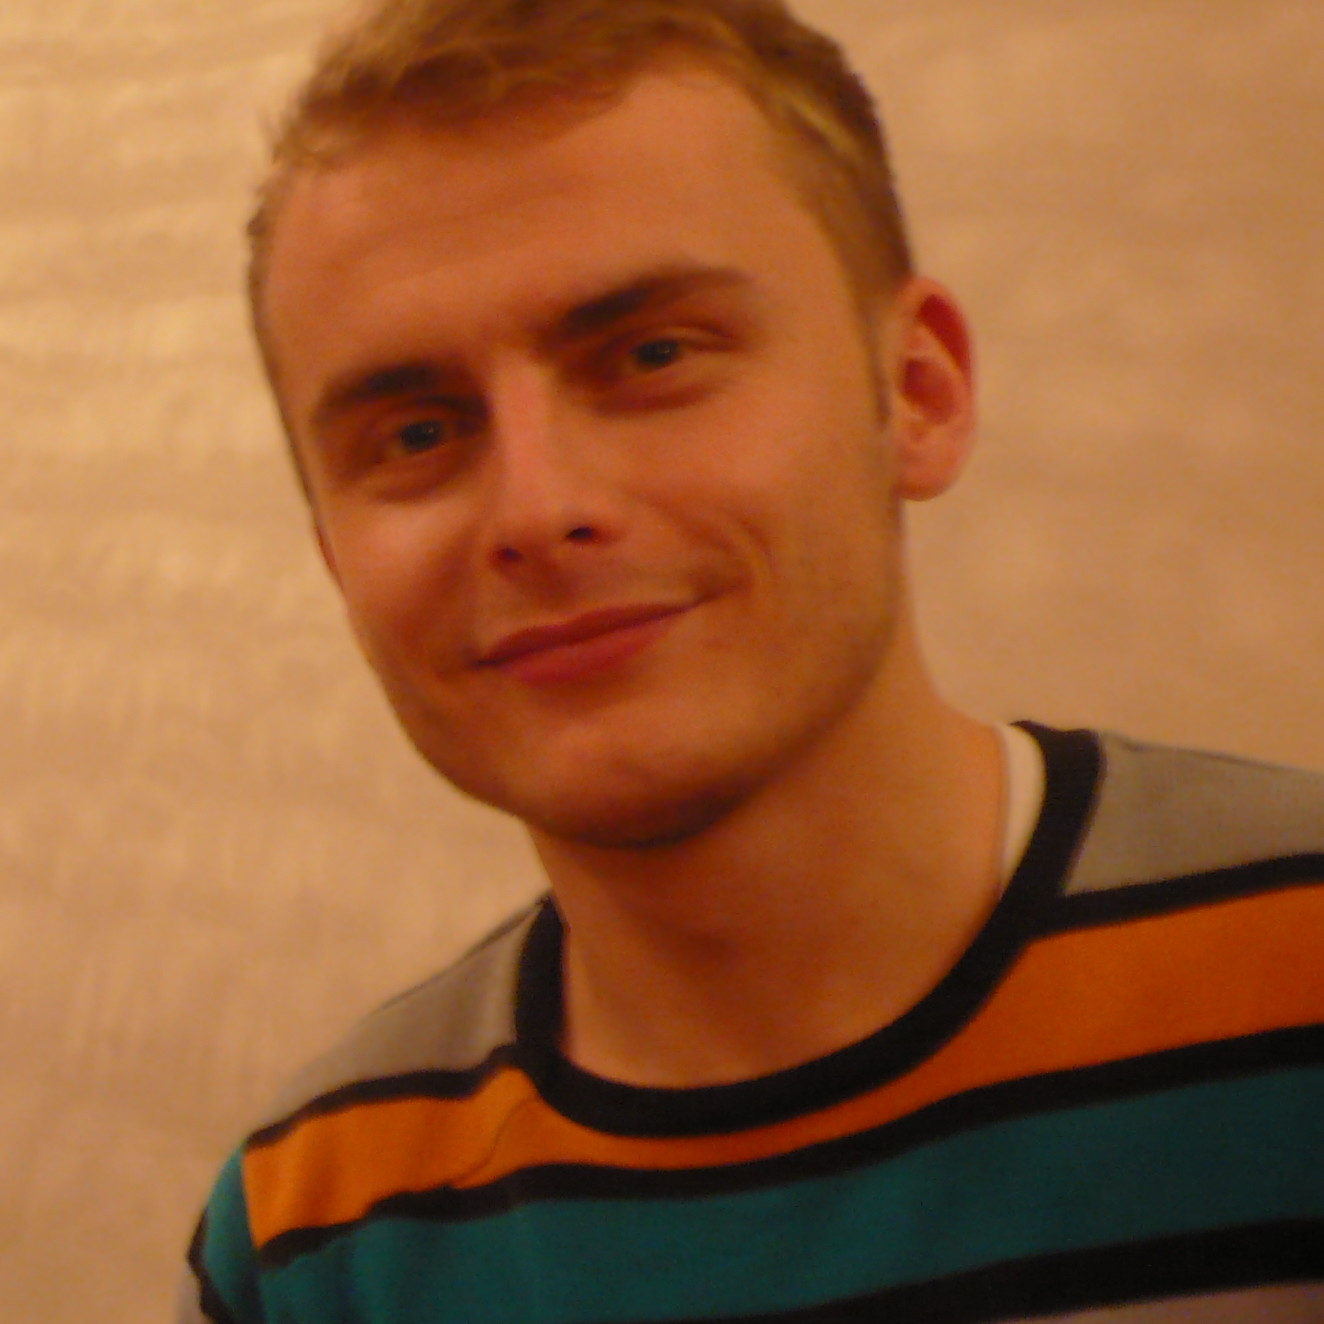
\includegraphics[width=0.075\textheight]{LinusSchumacher.jpg} \\
      
\includegraphics[width=0.075\textheight]{qrcode.png}
      \end{tabular}
 }
 % Title
 {{\sf\color{oxfordblue} Dynamics of leader-follower transitions in neural crest cell migration.}} 
 % Authors
 {\color{oxfordblue}Linus J.~Schumacher$^{1,2}$, R.~McLennan$^3$, J.A.~Morrison$^3$, J.M.~Teddy$^3$, D.~Kay$^2$, P.K.~Maini$^1$, R.E.~Baker$^1$ \& P.M.~Kulesa$^3$\\
 \texttt{\color{oxfordblue}schumacher@maths.ox.ac.uk, rem@stowers.org}\\
\textsl{\small 1: Wolfson Centre for Mathematical Biology, University of Oxford. 2: Computational Biology Group, University of Oxford. 3: Stowers Institute for Medical Research, Kansas City.}}
 % University logo
  { \begin{tabular}{r}%
 \raisebox{-1em}{
\includegraphics[width=0.1\textheight]{wcmb_logo2}}\\%
 {
\includegraphics[width=0.06\textheight]{LSI_hexagon_150mm}} %
 \raisebox{1.5em}{\includegraphics[width=0.05\textheight]{ox_brand_cmyk_rev}}%
 \end{tabular}
 }

%%%%%%%%%%%%%%%%%%%%%%%%%%%%%%%%%%%%%%%%%%%%%%%%%
%%% Now define the boxes that make up the poster
%%%---------------------------------------------------------------------------
%%% Each box has a name and can be placed absolutely or relatively.
%%% The only inconvenience is that you can only specify a relative position 
%%% towards an already declared box. So if you have a box attached to the 
%%% bottom, one to the top and a third one which should be in between, you 
%%% have to specify the top and bottom boxes before you specify the middle 
%%% box.
%%%%%%%%%%%%%%%%%%%%%%%%%%%%%%%%%%%%%%%%%%%%%%%%%

  \headerbox{Abstract}{name=background,column=0,row=0,span=2}{
	Neural crest cell migration is an important feature of vertebrate development and an emerging system for metastatic invasion. Mechanistic insight into the dynamics of intercellular and cell-microenvironmental interactions underlying this long-distance migration, however, has remained incomplete, particularly in mammalian and closely related avian model systems.
We study how leading and trailing subpopulations of cells are determined in the chick cranial neural crest. These cell subtypes are thought to be induced by different microenvironmental cues and to transmit directional information between each other. We interrogate our hypotheses about the main cue, vascular endothelial growth factor (VEGF), using a combination of \emph{in vivo}, \emph{in vitro} and computational experiments.
First we present a new, simple hypothesis for the phenotypic switching between leader and follower cell behaviour. To test the timescale of this transition, we measure gene expression of neural crest cells over time after removal of and re-exposure to VEGF. These results, in turn, are used to parametrise our model simulations. Next, we test the capacity of exogenous VEGF to change cell type and re-route migration, as well as the effect of removing endogenous VEGF from the lead and trailing subpopulations separately. In each case, we pair \emph{in vivo} experiments with model simulations that implement and test our hypotheses for their ability to produce the observed outcomes. }  
	
  \headerbox{Fig.\ 1: Response of gene expression to VEGF}{name=Fig1,column=0,below=background,span=1}{
	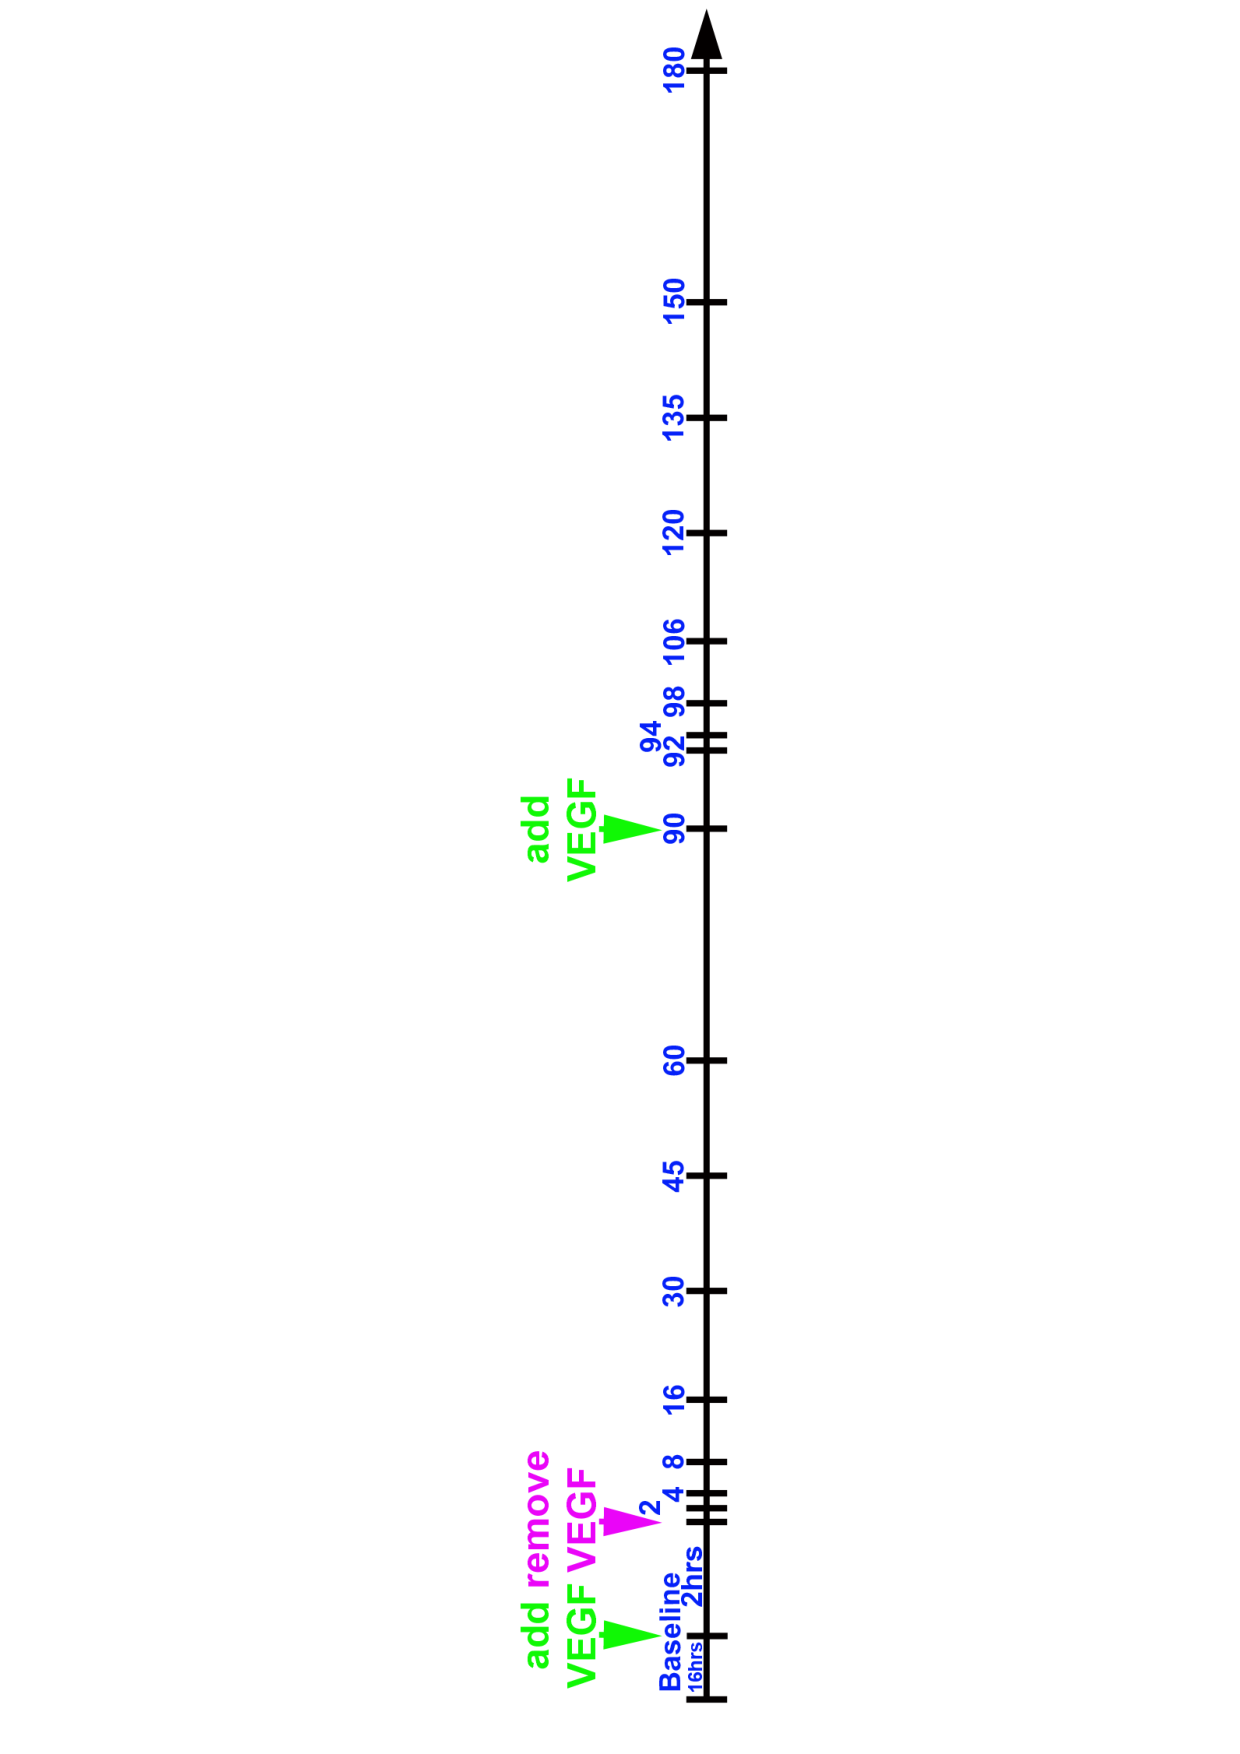
\includegraphics[trim=225 25 200 0, clip, scale=0.26,angle=270]{experiment}
	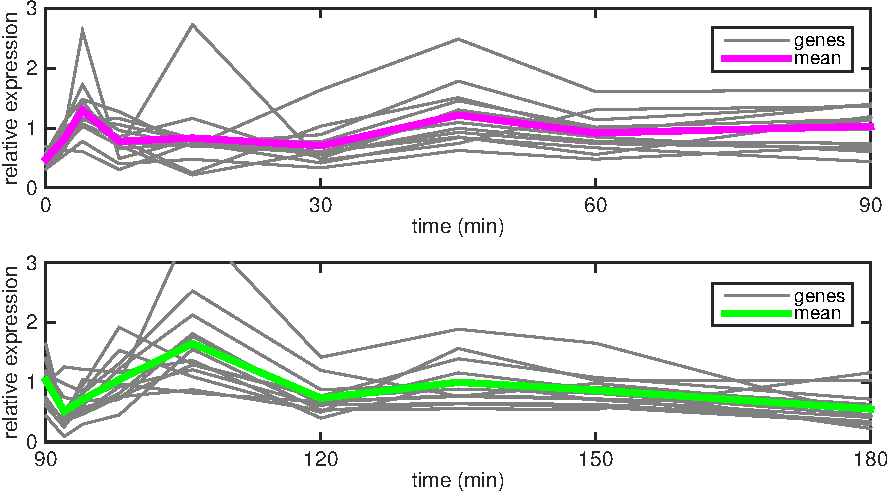
\includegraphics[scale=0.49]{significantGenes}}
	
  \headerbox{Fig.\ 2: Timing of first significant responses}{name=Fig2,column=0,below=Fig1,span=1}{
	\includegraphics[scale=0.575]{responseTimes}}
	
\headerbox{Fig.\ 3: Timecourse of early-response genes}{name=Fig3,column=0,below=Fig2,span=1}{
	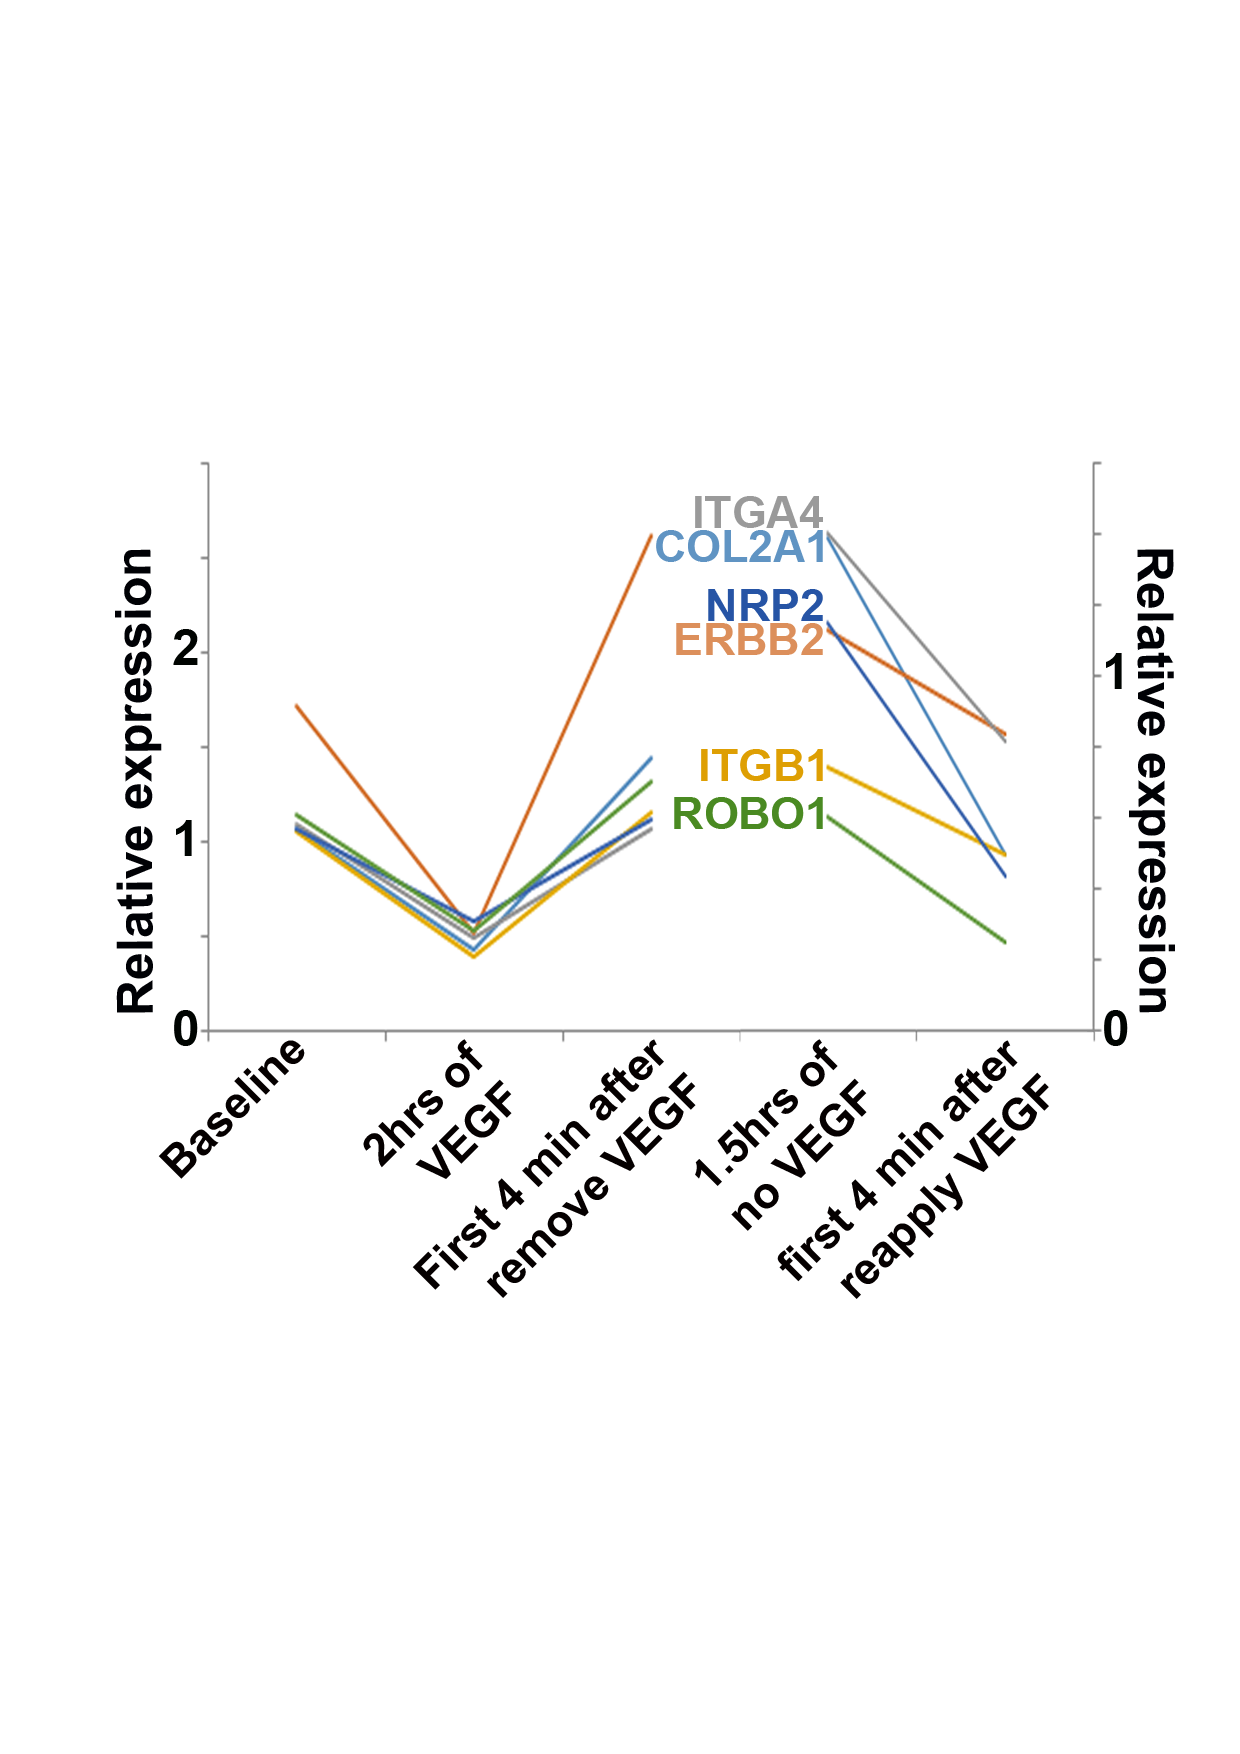
\includegraphics[trim=35 197 0 210, clip, scale=0.375]{4minGenes}}
	
\headerbox{Fig.\ 4: ``Integrate and switch'' model}{name=Fig4,column=1,below=background,span=1}{
	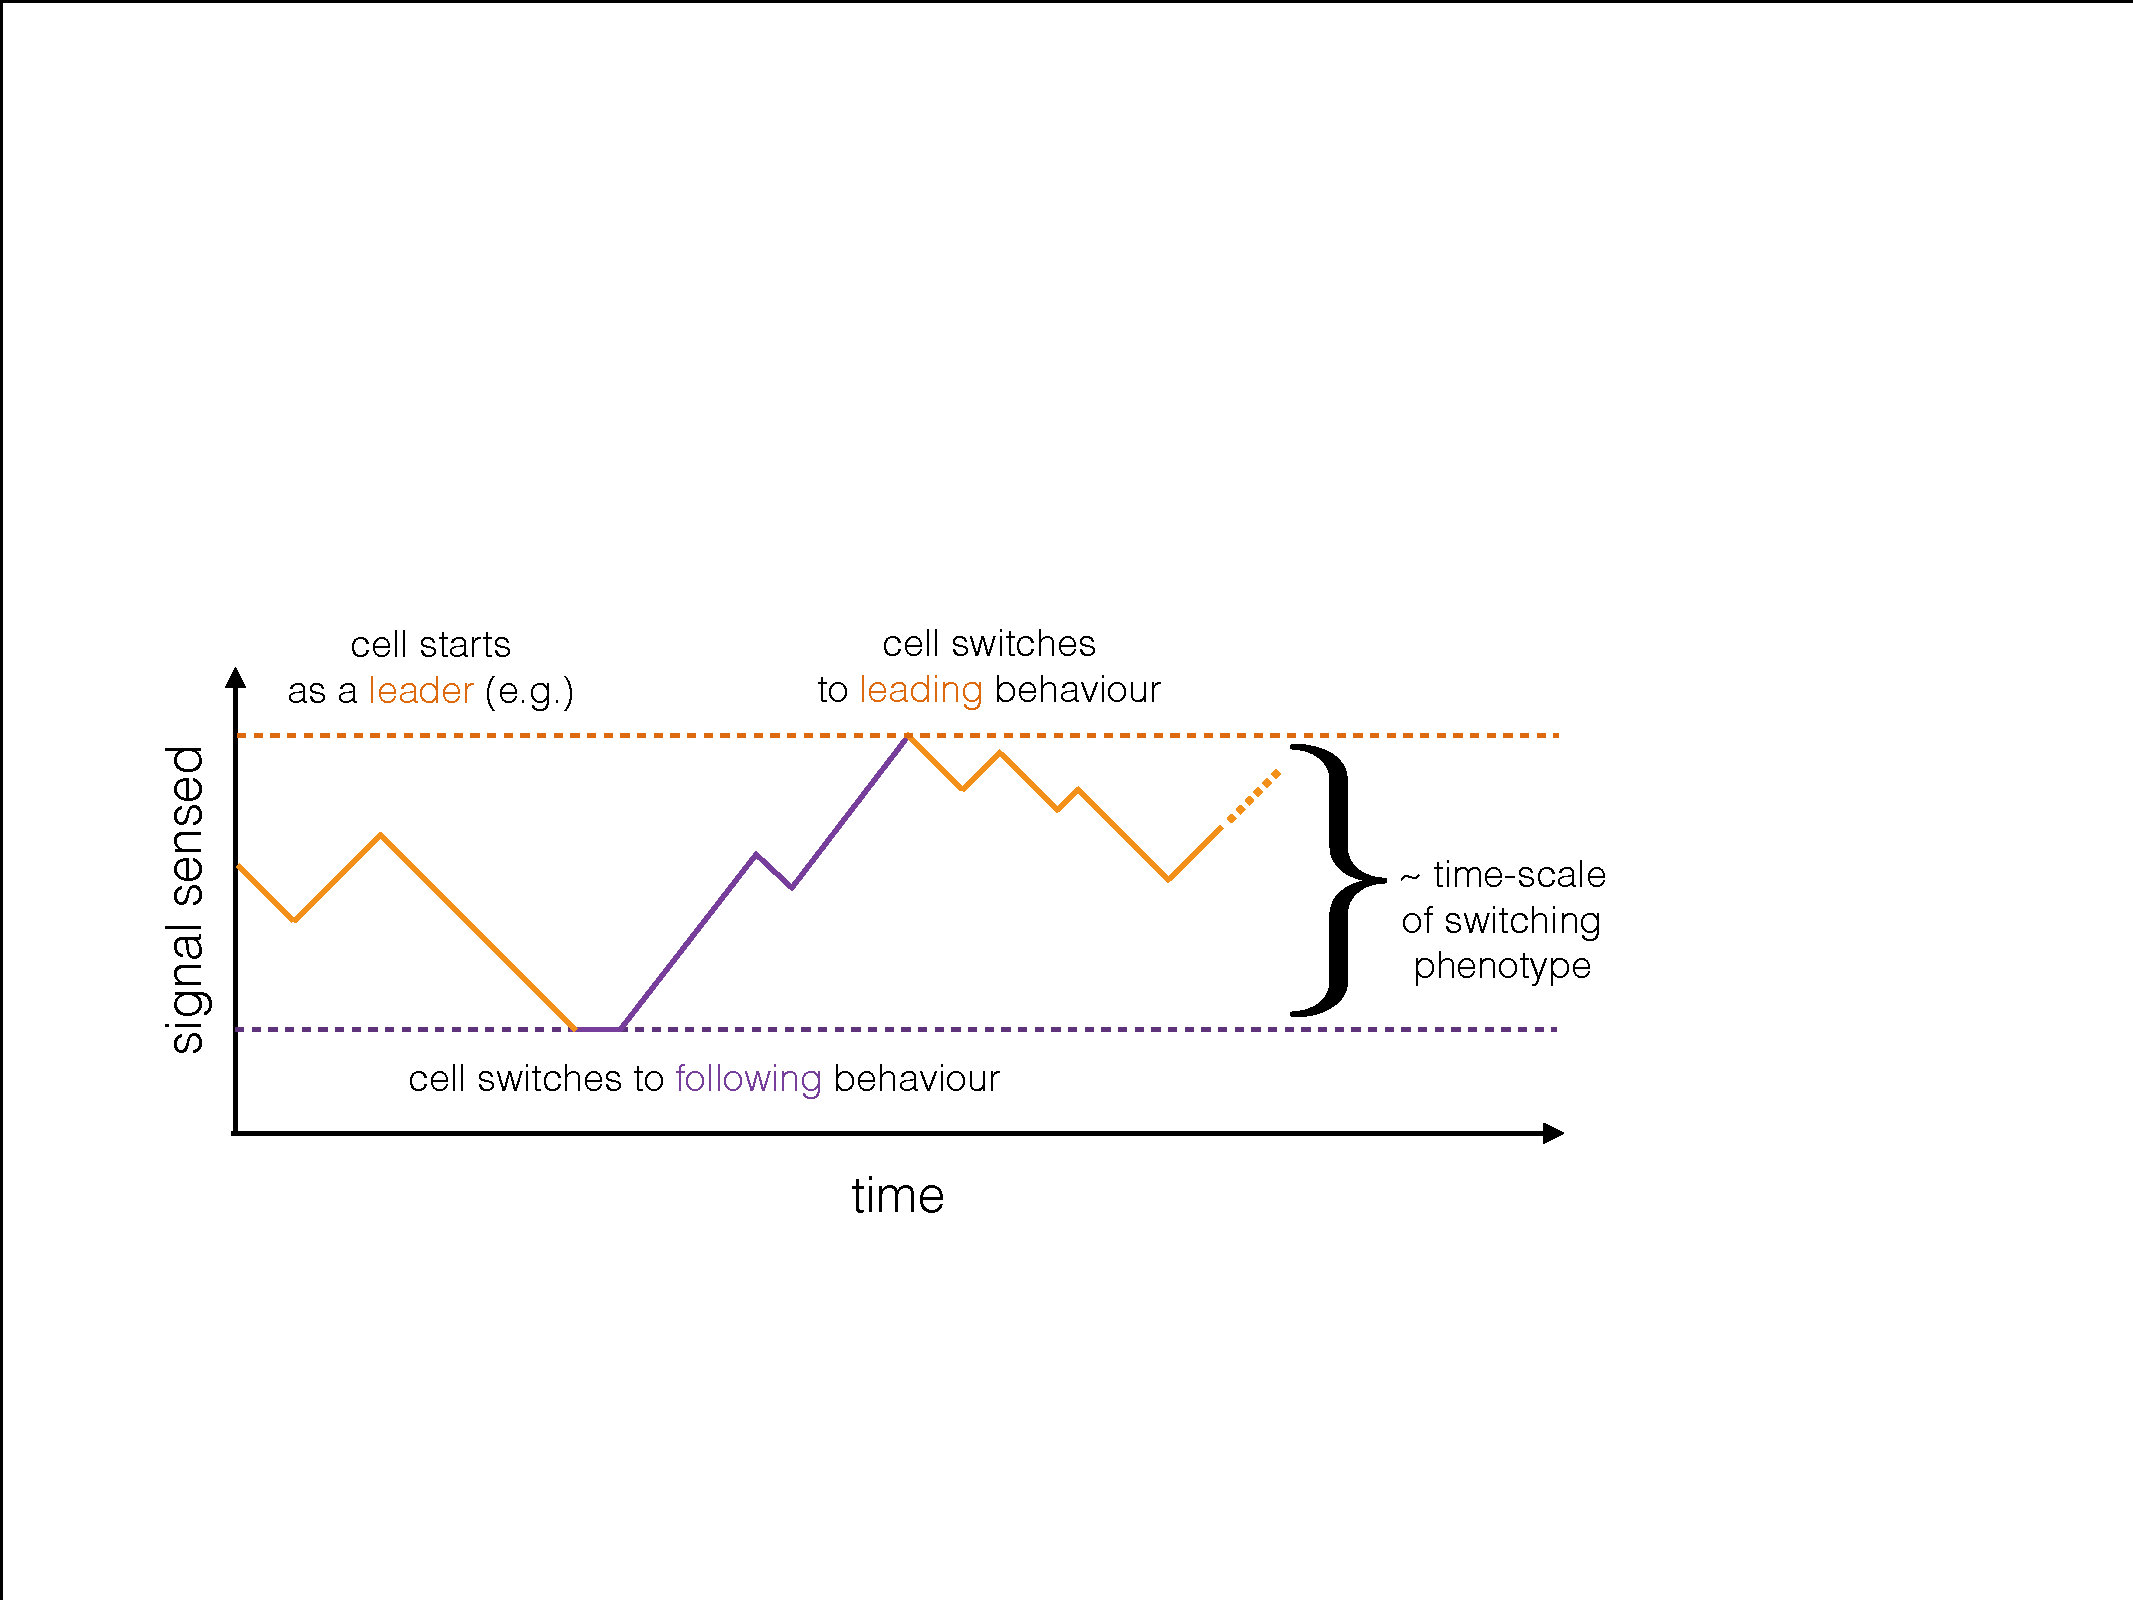
\includegraphics[trim=79 160 253 270, clip,scale=0.305]{ISmodel}}  
	
\headerbox{Fig.\ 5: Trailing neural crest cells respond to ectopic VEGF in \emph{in vivo} and computational experiments}{name=Fig5,column=1,below=Fig4,span=2}{
	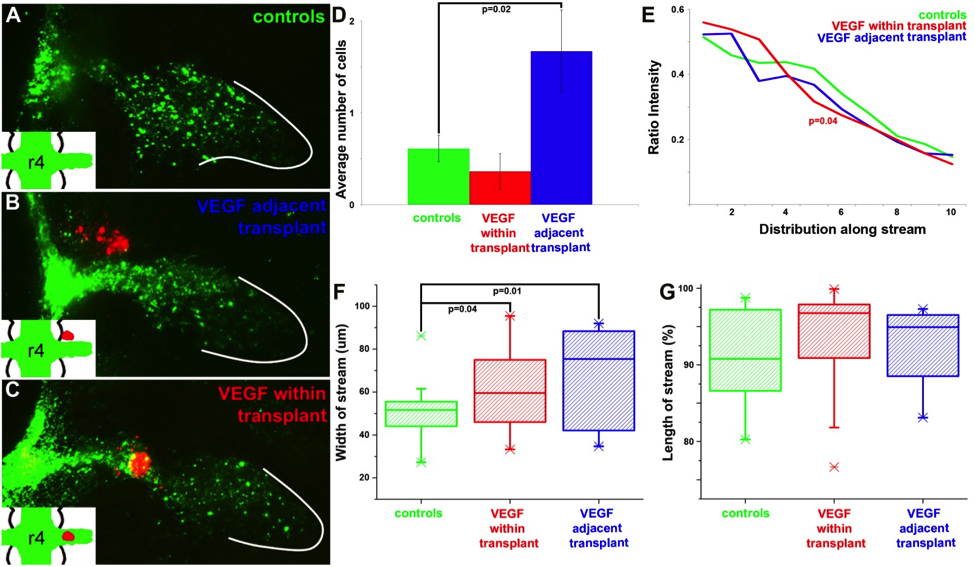
\includegraphics[trim=10 00 162 0, clip,scale=0.7]{reroute}
	\begin{minipage}{250pt}
	\vspace*{-175pt}
	\hspace*{3pt} Model simulation control\hspace*{20pt} \includegraphics[scale=0.5]{fig5key}\\[-5pt]
	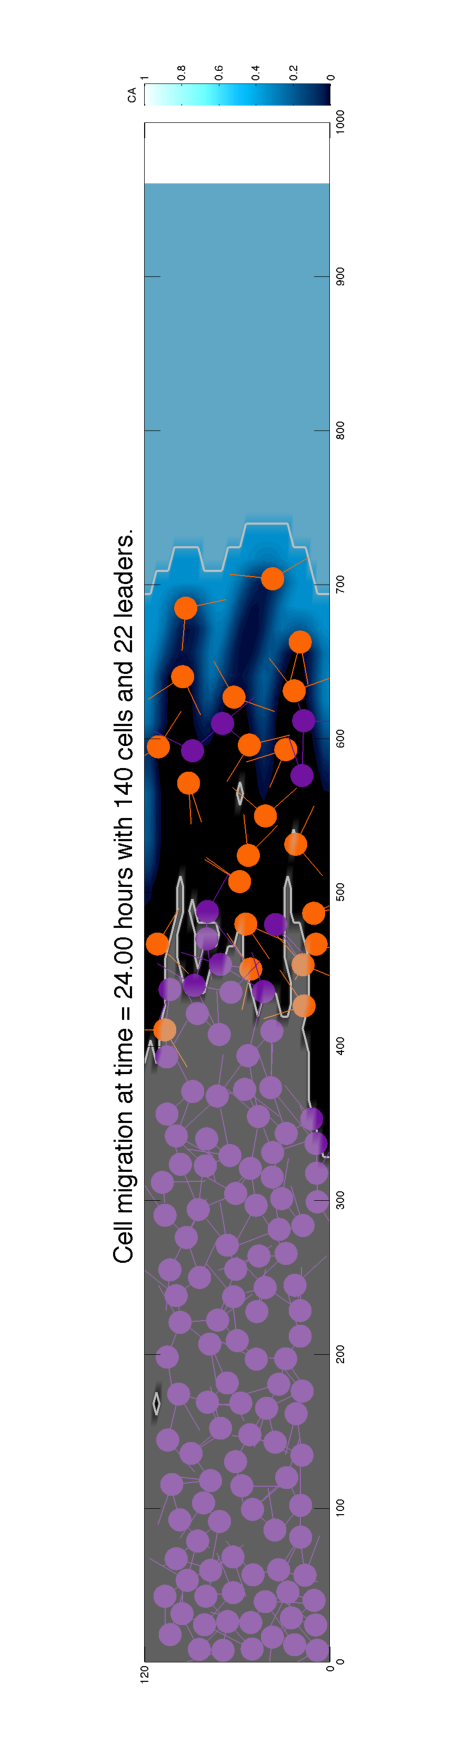
\includegraphics[trim=68 30 25 200, clip,scale=0.35,angle=270]{modelControl-crop}\\%
	\hspace*{3pt} Increased chemoattractant at lower left boundary\\[-5pt]
	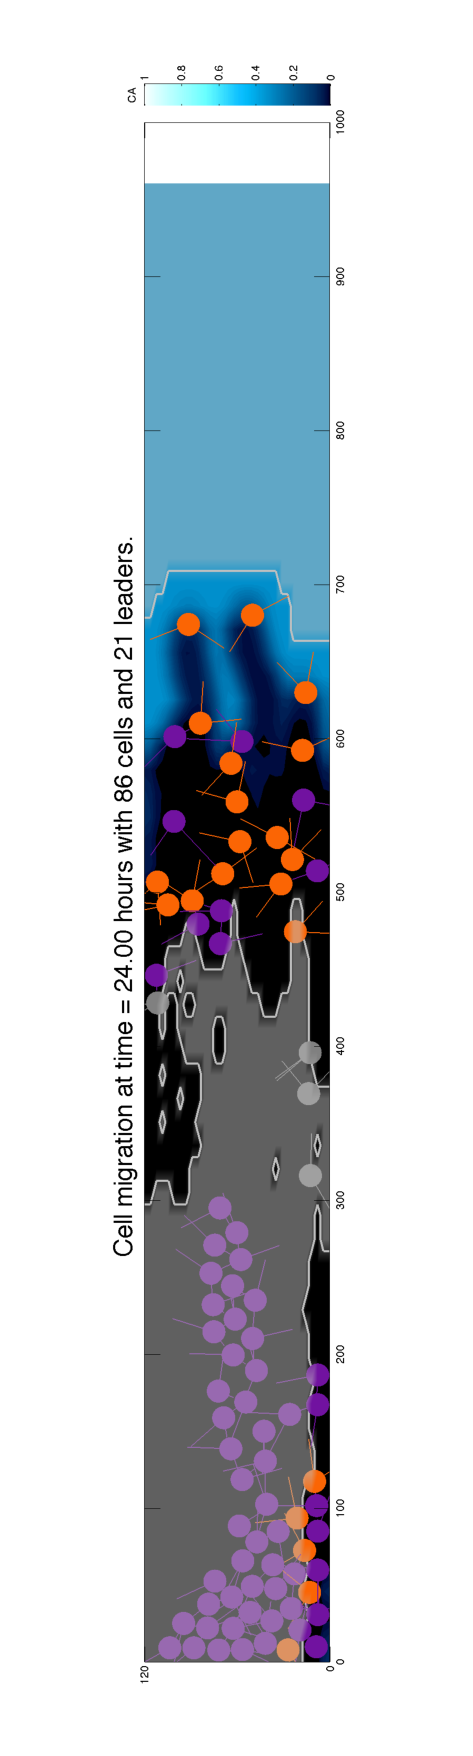
\includegraphics[trim=68 30 25 200, clip,scale=0.35,angle=270]{modelAdjacent-crop}\\%
	\hspace*{3pt} Increased chemoattractant in lower left area\\[-5pt]
	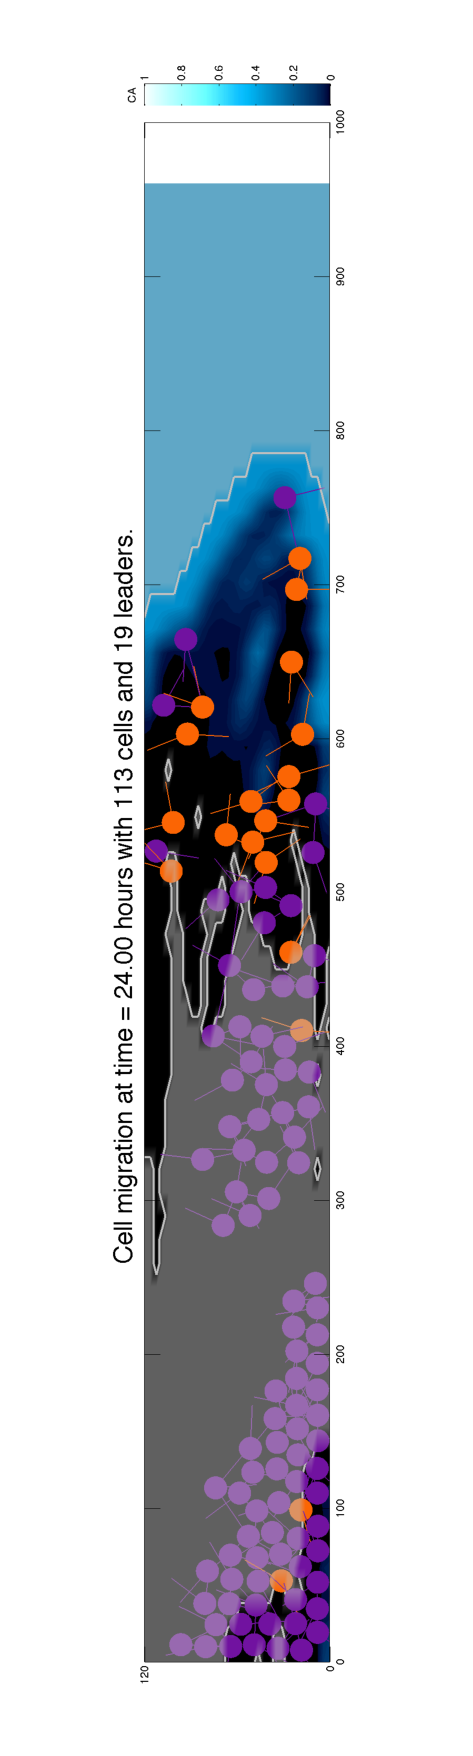
\includegraphics[trim=68 30 40 200, clip,scale=0.35,angle=270]{modelWithinBack-crop}%
	\end{minipage}
	\vspace*{-7pt}
	}  

\headerbox{Fig.\ 6: Trailing cells migrate independent of VEGF}{name=Fig6,column=1,below=Fig5,span=1}{
	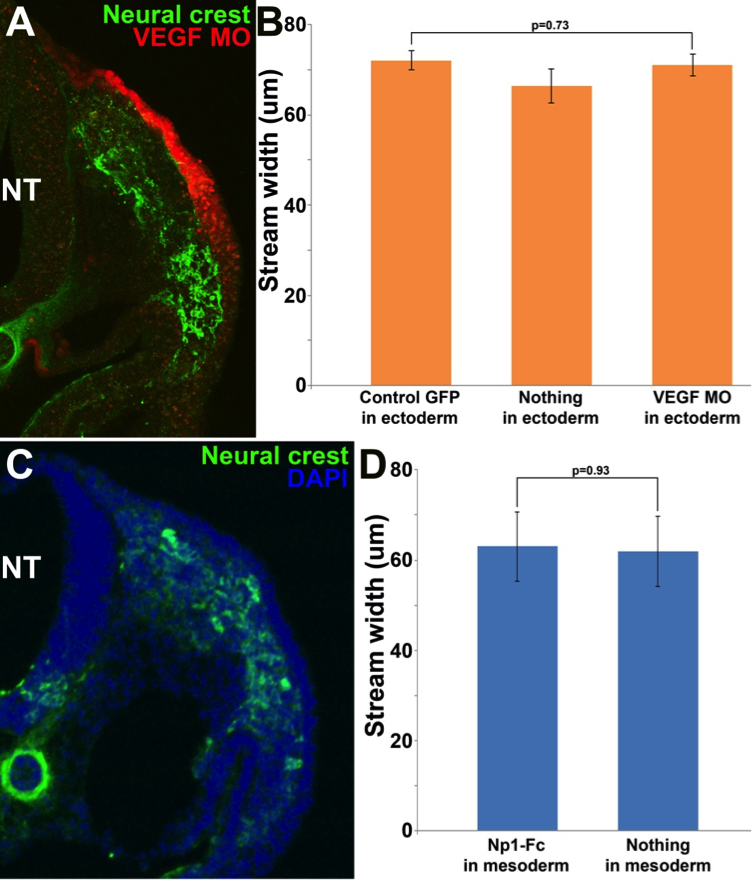
\includegraphics[trim=-50 0 0 0, clip,scale=0.45]{noVEGF}}  
		
\headerbox{Discussion and Conclusion}{name=discussion,column=2,row=0,span=1}{
\begin{itemize}
	\item Neural crest cells grown in culture have different molecular profiles to those in the embryo.
	\item The molecular profiles of neural crest cells in culture respond to changes in VEGF within minutes (Fig.~1-3).
	\item Ectopic sources of VEGF can disrupt stream migration. Trailing cells cluster, lead cells migrate onwards (Fig.~5).
	\item Consistent with our hypothesis and model, VEGF is not necessary for collective migration of trailing cells (Fig.~6).
 	\item[$\rightarrow$] VEGF is one of the embryonic microenvironmental signals guiding migration and driving lead neural crest cell identity.
 \end{itemize}
	}
	
	
\headerbox{Acknowledgements}{name=acknowledgements,column=2,below=discussion,span=1}{LJS would like to thank Louise Dyson for helpful discussions and access to the  code from \cite{McLennan2012} and gratefully acknowledges the U.K.\ Engineering and Physical Sciences Research Council for funding through a studentship at the Life Science Interface Doctoral Training Centre of  the University of Oxford.
	\vspace{0.1cm}
}

% %%%%%%%%%%%%%%%%%%%%%%%%%%%%%%%%%%%%%%%%%%%%%%%% 
 \headerbox{References}{name=references,column=2,below=Fig5}{
 %%%%%%%%%%%%%%%%%%%%%%%%%%%%%%%%%%%%%%%%%%%%%%%%%
     \smaller
     
     \bibliographystyle{unsrt}
     \renewcommand{\section}[2]{\vskip 0.05em}
       \begin{thebibliography}{1}\itemsep=-0.01em
       \setlength{\baselineskip}{0.4em}
	
	\bibitem{McLennan2010}
	R.\ McLennan, J.M.\ Teddy, J.C.\ Kasemeier-Kulesa, M.H.\ Romine \& P.M.\ Kulesa
	\newblock{Vascular Endothelial Growth Factor Regulates Cranial Neural Crest Migration \emph{in vivo}}.
	\newblock{\em Developmental Biology}, 339(1), pp.114-125, (2010).

	 \bibitem{McLennan2012}
	R.\ McLennan, L.\ Dyson*, K.W.\ Prather, J.A.\ Morrison, R.E.\ Baker, P.K.\ Maini \& P.M. Kulesa.
	\newblock {Multiscale mechanisms of cell migration during development: theory and experiment}.
	\newblock {\em Development}, 16, pp.2935-44, (2012).

	\bibitem{profiling}
	R.\ McLennan, L.J.\ Schumacher*, J.A.\ Morrison, J.M.\ Teddy, D.\ Ridenour, A.\ Box, C.\ Semerad, H.\ Li, W.\ McDowell, D.\ Kay, P.K.\ Maini, R.E.\ Baker \& P.M.\ Kulesa.
	\newblock {Neural Crest migration is driven by a few trailblazer cells with a unique molecular signature narrowly confined to the invasive front}.
	\newblock {\em In preparation}

	\bibitem{VEGFfollowup}
	R.\ McLennan, L.J.\ Schumacher, J.A.\ Morrison, J.M.\ Teddy, D.\ Kay, P.K.\ Maini, R.E.\ Baker \& P.M.\ Kulesa.
	\newblock {VEGF is one of the embryonic microenvironmental drivers of trailblazer neural crest cell identity}.
	\newblock {\em In preparation}
	
       	\vspace*{4pt}

       \end{thebibliography}
   }

 %%%%%%%%%%%%%%%%%%%%%%%%%%%%%%%%%%%%%%%%%%%%%%%%%    
 \end{poster}%
%
\end{document}
